\documentclass{article}

\usepackage{arxiv}

\usepackage[utf8]{inputenc} % allow utf-8 input
\usepackage[T1]{fontenc}    % use 8-bit T1 fonts
\usepackage{hyperref}       % hyperlinks
\usepackage{url}            % simple URL typesetting
\usepackage{booktabs}       % professional-quality tables
\usepackage{amsfonts}       % blackboard math symbols
\usepackage{nicefrac}       % compact symbols for 1/2, etc.
\usepackage{microtype}      % microtypography
\emergencystretch=1em       % suppress underfull hbox warnings
\usepackage{lipsum}         % Can be removed after putting your text content
\usepackage{graphicx}
\usepackage{natbib}
\usepackage{doi}
\usepackage{amsmath}
\usepackage{cleveref}       % smart cross-referencing (must be after amsmath)
\usepackage{ulem}
\usepackage{tikz}
\usetikzlibrary{positioning, arrows.meta, fit, backgrounds, shapes.geometric, decorations.pathreplacing}
\usepackage{amsthm}
\usepackage{algorithm}
\usepackage{algpseudocode}
\usepackage{listings}
\lstset{
  language=Python,
  basicstyle=\ttfamily\footnotesize,
  keywordstyle=\bfseries\color{blue!70!black},
  commentstyle=\itshape\color{gray},
  stringstyle=\color{red!60!black},
  breaklines=true,
  frame=single,
  framerule=0.4pt,
  rulecolor=\color{gray!40},
  xleftmargin=1em,
  xrightmargin=0.5em,
  aboveskip=0.8em,
  belowskip=0.5em,
  showstringspaces=false,
}
\usepackage{xcolor}

\theoremstyle{definition}
\newtheorem{definition}{Definition}[section]
\newtheorem{remark}{Remark}[section]

% Notation shorthands
\newcommand{\LT}{\mathbf{LT}}
\newcommand{\MD}{\mathbf{MD}}
\newcommand{\BBox}{\mathcal{B}}
\newcommand{\Nodes}{\mathcal{N}}
\newcommand{\Spans}{\mathcal{S}}

\newcommand{\todo}{\textcolor{red}{TODO}}

\title{Multimodal Document Alignment: Bridging Visual Layout Trees and OCR-Extracted Text}

% Here you can change the date presented in the paper title
\date{April, 2026}
% Or remove it
%\date{}

\newif\ifuniqueAffiliation
% Comment to use multiple affiliations variant of author block
\uniqueAffiliationtrue

\ifuniqueAffiliation % Standard variant of author block
\author{
  {Levi Willms}
  \thanks{
    This document is a partial fulfillment of the requires for the Undergraduate honours thesis in Computer Science.
  } \\
  Computer Science, Faculty of Science\\
  Ontario Tech University\\
  Oshawa, ON \\
  \texttt{levi.willms@ontariotechu.net} \\
  \And
  {Ken Pu (\textsc{Supervisor})} \\
  Computer Science, Faculty of Science\\
  Ontario Tech University\\
  Oshawa, ON \\
  \texttt{ken.pu@ontariotechu.ca} \\
}
\else
% Multiple affiliations variant of author block
\usepackage{authblk}
\renewcommand\Authfont{\bfseries}
\setlength{\affilsep}{0em}
% box is needed for correct spacing with authblk
\newbox{\orcid}\sbox{\orcid}{\includegraphics[scale=0.06]{orcid.pdf}}
\author[1]{%
  \href{https://orcid.org/0000-0000-0000-0000}{\usebox{\orcid}\hspace{1mm}David S.~Hippocampus\thanks{\texttt{hippo@cs.cranberry-lemon.edu}}}%
}
\author[1,2]{%
  \href{https://orcid.org/0000-0000-0000-0000}{\usebox{\orcid}\hspace{1mm}Elias D.~Striatum\thanks{\texttt{stariate@ee.mount-sheikh.edu}}}%
}
\affil[1]{Department of Computer Science, Cranberry-Lemon University, Pittsburgh, PA 15213}
\affil[2]{Department of Electrical Engineering, Mount-Sheikh University, Santa Narimana, Levand}
\fi

% Uncomment to override  the `A preprint' in the header
\renewcommand{\headeright}{Honours thesis}
\renewcommand{\undertitle}{}
\renewcommand{\shorttitle}{}

%%% Add PDF metadata to help others organize their library
%%% Once the PDF is generated, you can check the metadata with
%%% $ pdfinfo template.pdf
\hypersetup{
  pdftitle={},
  pdfsubject={},
  pdfauthor={},
  pdfkeywords={},
}

\begin{document}
\maketitle

\begin{abstract}
  \textbf{Problem.}
  \begin{itemize}
    \item A document page image yields two parallel representations:
          \begin{itemize}
            \item \emph{Visual tokens} --- labelled bounding boxes organised into a
                  hierarchical Layout Tree $\mathbf{LT}$
            \item \emph{Text tokens} --- natural-language tokens of the OCR-generated
                  Markdown document $\mathbf{MD} \in \mathbf{Char}^{*}$
          \end{itemize}
    \item Each view alone is incomplete; neither carries the full semantics of the page.
    \item \textbf{Goal:} assign every node of $\mathbf{LT}$ a contiguous, monotone span
          of $\mathbf{MD}$ --- the \emph{layout-text alignment problem}.
  \end{itemize}

  \medskip
  \textbf{Contributions.}
  \begin{enumerate}
    \item \textbf{Formal model} --- cast alignment as a monotone interval-partition task;
          exact solution via dynamic programming in $O(nL^{2})$ time.
    \item \textbf{Hybrid aligner} --- exact DP for short token sequences ($L \le 100$),
          greedy $O(nL)$ approximation for long documents; accuracy preserved within
          practical time budgets.
    \item \textbf{Composable pipeline} --- type-safe Python library on PaddleOCR /
          PPStructure\,V3, with Pandera-validated intermediate representations, making
          every stage inspectable and reusable.
  \end{enumerate}
\end{abstract}

% keywords can be removed
\keywords{document understanding \and layout analysis \and OCR \and sequence alignment \and
  multimodal document processing}

% Sections go here

%% ---------------------------------------------------------------
\section{Introduction}
%% ---------------------------------------------------------------
\begin{itemize}
  \item OCR converts document images to text but discards spatial structure
        \cite{ieee2025systematic}
  \item Document layout analysis recovers spatial structure as labelled bounding boxes
        \cite{PPDocLayout}
  \item The two modalities are complementary; neither is sufficient alone
  \item This work bridges them via a principled alignment framework powered by
        PaddleOCR / PPStructure\,V3 \cite{PaddleOCR30}
\end{itemize}

%% ---------------------------------------------------------------
\section{Related Work}
%% ---------------------------------------------------------------

\subsection{Optical Character Recognition}
\begin{itemize}
  \item Progression from rule-based to deep-learning OCR engines
        \cite{ieee2025systematic, yao2025analysis}
  \item PP-OCRv3: lightweight, high-accuracy OCR backbone \cite{PaddleOCRv3}
  \item PaddleOCR 3.0: full pipeline including layout parsing \cite{PaddleOCR30}
  \item PaddleOCR-VL: vision-language model for multilingual document parsing
        \cite{paddleocrvl2025}
\end{itemize}

\subsection{Document Layout Analysis}
\begin{itemize}
  \item PP-DocLayout: unified detection model for large-scale data construction
        \cite{PPDocLayout}
  \item DLAFormer: end-to-end transformer for layout analysis \cite{wang2024dlaformer}
  \item SFDLA: source-free domain adaptation for layout analysis \cite{tewes2025sfdla}
  \item SCAN: semantic layout analysis for retrieval-augmented generation
        \cite{scan2025semantic}
  \item Graph-based document structure analysis \cite{gdsa2025graph}
\end{itemize}

\subsection{Reading Order and Structure Extraction}
\begin{itemize}
  \item Modeling layout reading order as ordering relations \cite{zhang2024modeling}
  \item \'{E}clair: integrated content, layout, and reading-order extraction
        \cite{eclair2025extracting}
\end{itemize}

%% ---------------------------------------------------------------
\section{Problem Formulation}
%% ----------------------------------------------------------------

\subsection{Document Representations}

\begin{definition}[Raster Document]
  A \emph{raster document} is a finite sequence of page images
  $D = \langle d_1, d_2, \ldots, d_P \rangle$, where each page
  $d_p \in \mathbb{R}^{H \times W \times 3}$ is an RGB image of height $H$
  and width $W$.  All subsequent definitions apply to a single page; the
  page index $p$ is dropped for brevity.
\end{definition}

\begin{definition}[Bounding Box]
  A \emph{bounding box} over a label set $\Lambda$ is a tuple
  \[
    b = (x_0,\, y_0,\, x_1,\, y_1,\, \lambda)
    \;\in\; \mathbb{N}^4 \times \Lambda,
  \]
  where $(x_0, y_0)$ is the top-left corner, $(x_1, y_1)$ is the
  bottom-right corner, and $\lambda \in \Lambda$ is the semantic label
  (e.g.\ \texttt{paragraph}, \texttt{figure}, \texttt{table}).
  The \emph{area} of $b$ is $\mathrm{area}(b) = (x_1 - x_0)(y_1 - y_0)$.
\end{definition}

\begin{definition}[Containment]
  Bounding box $b'$ is \emph{contained in} $b$, written $b' \sqsubseteq b$,
  if and only if
  \[
    \frac{\mathrm{area}(b \cap b')}{\mathrm{area}(b')} \;\ge\; \tau,
  \]
  for a fixed tolerance $\tau \in (0, 1]$, where $b \cap b'$ denotes the
  rectangular intersection.  We use $\tau = 0.8$ throughout.
\end{definition}

\subsection{Visual Tokens and the Layout Tree}

\begin{definition}[Visual Token Layers]
  A document page is analysed into four ordered token layers:
  \begin{itemize}
    \item $R = \{r_i\}$ --- \emph{region} bounding boxes (coarsest granularity)
    \item $K = \{k_j\}$ --- \emph{block} bounding boxes, each assigned a reading
          order index $\mathrm{ord}(k_j) \in \mathbb{N}$
    \item $\ell = \{\ell_m\}$ --- \emph{line} bounding boxes, sorted by $y_0$
    \item $W = \{w_n\}$ --- \emph{word} bounding boxes, grouped by line membership
  \end{itemize}
\end{definition}

\begin{definition}[Layout Tree]
  \label{def:lt}
  The \emph{Layout Tree} $\LT$ is a rooted tree whose node set is
  $\Nodes = R \cup K \cup \ell \cup W$ and whose edges encode containment:
  \[
    \mathrm{parent}(v) = \arg\max_{u \in \mathrm{level}(v)-1}
    \frac{\mathrm{area}(u \cap v)}{\mathrm{area}(v)},
  \]
  where $\mathrm{level}(v) \in \{0,1,2,3\}$ denotes region, block, line, and
  word respectively.  Children of each internal node are sorted by reading
  order \cite{zhang2024modeling}.  See \cref{fig:layout-tree}.
\end{definition}

\begin{figure}[h]
  \centering
  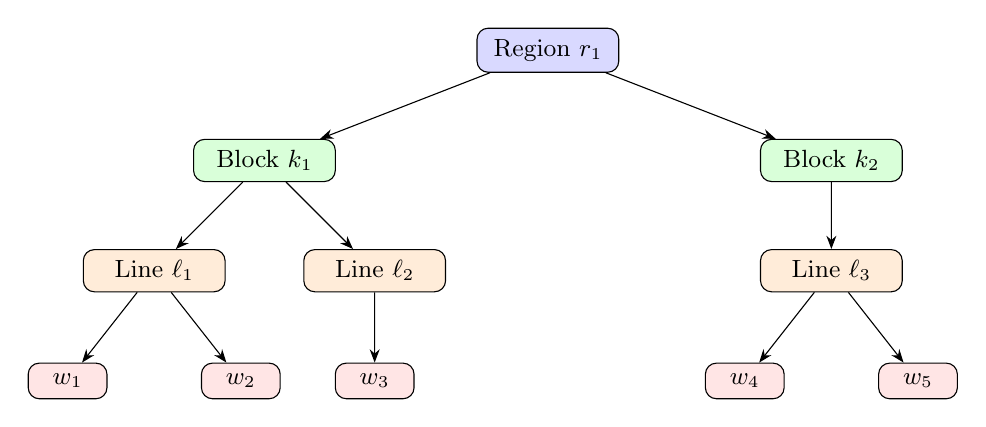
\begin{tikzpicture}[
      level distance=14mm,
      level 1/.style={sibling distance=72mm},
      level 2/.style={sibling distance=28mm},
      level 3/.style={sibling distance=22mm},
      every node/.style={draw, rounded corners, font=\small,
          inner sep=4pt, minimum width=18mm},
      region/.style={fill=blue!15},
      block/.style={fill=green!15},
      line/.style={fill=orange!15},
      word/.style={fill=red!10, minimum width=10mm},
      edge from parent/.style={draw, ->, >=Stealth},
    ]
    \node[region] {Region $r_1$}
    child { node[block] {Block $k_1$}
        child { node[line] {Line $\ell_1$}
            child { node[word] {$w_1$} }
            child { node[word] {$w_2$} }
          }
        child { node[line] {Line $\ell_2$}
            child { node[word] {$w_3$} }
          }
      }
    child { node[block] {Block $k_2$}
        child { node[line] {Line $\ell_3$}
            child { node[word] {$w_4$} }
            child { node[word] {$w_5$} }
          }
      };
  \end{tikzpicture}
  \caption{Schematic of the Layout Tree $\LT$.  Colours denote hierarchy
    levels: \textcolor{blue!60}{region} $\supset$
    \textcolor{green!60!black}{block} $\supset$
    \textcolor{orange!80!black}{line} $\supset$
    \textcolor{red!60}{word}.
    Children within each level are ordered by reading order.}
  \label{fig:layout-tree}
\end{figure}

\subsection{Text Tokens and the Markdown Document}

\begin{definition}[Text Token Sequence]
  An OCR engine applied to $d$ produces a \emph{Markdown document}
  $\MD \in \Sigma^{*}$, where $\Sigma$ is the Unicode character set.
  Tokenising $\MD$ with a word tokeniser yields an ordered sequence
  \[
    T = \langle t_0,\, t_1,\, \ldots,\, t_{L-1} \rangle,
    \quad t_i \in \Sigma^{+}.
  \]
  Each token $t_i$ is associated with a character span
  $\sigma_i = [s_i, e_i) \subseteq [0, |\MD|)$.
  See \cref{fig:text-tokens}.
\end{definition}

\begin{definition}[Token Span]
  A \emph{token span} is a half-open integer interval
  $[a, b) \subseteq [0, L)$ with $a \le b$.
  The \emph{sub-sequence} induced by $[a,b)$ is
  $T[a:b] = \langle t_a, t_{a+1}, \ldots, t_{b-1} \rangle$.
\end{definition}

\begin{figure}[h]
  \centering
  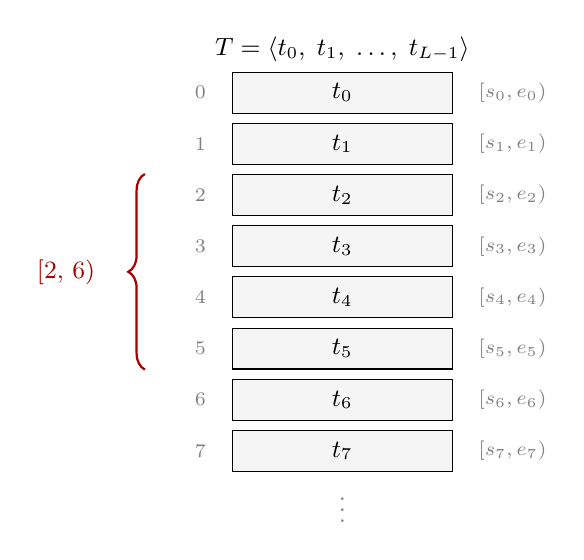
\begin{tikzpicture}[
      tok/.style={draw, fill=gray!8, font=\small, inner sep=3pt,
          minimum height=0.52cm, minimum width=2.8cm, text centered},
    ]
    % Header
    \node[font=\small\bfseries] (hdr) at (0, 0.55)
    {$T = \langle t_0,\; t_1,\; \ldots,\; t_{L-1} \rangle$};

    % Token boxes stacked vertically
    \foreach \i/\lab/\span in {
    0/$t_0$/{\scriptsize$[s_0,e_0)$},
      1/$t_1$/{\scriptsize$[s_1,e_1)$},
      2/$t_2$/{\scriptsize$[s_2,e_2)$},
      3/$t_3$/{\scriptsize$[s_3,e_3)$},
      4/$t_4$/{\scriptsize$[s_4,e_4)$},
      5/$t_5$/{\scriptsize$[s_5,e_5)$},
      6/$t_6$/{\scriptsize$[s_6,e_6)$},
      7/$t_7$/{\scriptsize$[s_7,e_7)$}}{
      \node[tok] (T\i) at (0, {-\i*0.65}) {\lab};
      % index on left
      \node[font=\scriptsize, gray, left=2mm of T\i] {\i};
      % character span on right
      \node[font=\scriptsize, gray, right=2mm of T\i] {\span};
      }

      % Brace showing an example token span [2,6)
      \draw[decorate,
        decoration={brace, amplitude=6pt, mirror},
        thick, red!65!black]
      ([xshift=-1.1cm]T2.north west) --
      ([xshift=-1.1cm]T5.south west)
      node[midway, left=5mm, font=\small, red!65!black] {$[2,\,6)$};

    % Trailing ellipsis
    \node[font=\small, gray] at (0, {-8*0.65}) {$\vdots$};
  \end{tikzpicture}
  \caption{The text token sequence $T$ produced by tokenising the OCR-generated
  Markdown $\MD$.  Tokens are indexed $0 \ldots L{-}1$ (left) and each
  carries a character-level span $[s_i, e_i)$ in $\MD$ (right).
  The red brace marks an example \emph{token span} $[2,6)$, selecting
  the contiguous sub-sequence $\langle t_2, t_3, t_4, t_5 \rangle$.}
  \label{fig:text-tokens}
\end{figure}

\subsection{The Alignment Problem}

\begin{definition}[Node Alignment]
  \label{def:alignment}
  A \emph{node alignment} is a function
  $\phi : \Nodes \to \Spans$
  that maps every layout node $v \in \Nodes$ to a token span
  $\phi(v) = [a_v, b_v)$.
  An alignment is \emph{valid} if it satisfies:
  \begin{enumerate}
    \item \textbf{Monotonicity.}
          For any two siblings $v, v'$ with $v \prec v'$ in reading order,
          $b_v \le a_{v'}$ (spans do not cross).
    \item \textbf{Containment.}
          For every parent--child pair $(u, v)$,
          $\phi(u) \supseteq \phi(v)$, i.e.\ $a_u \le a_v$ and $b_v \le b_u$.
    \item \textbf{Coverage.}
          The root $r$ satisfies $\phi(r) = [0, L)$ (all tokens are covered).
  \end{enumerate}
\end{definition}

\begin{definition}[Similarity Function]
  A \emph{similarity function} is a mapping
  $\mathrm{sim} : \Nodes \times \Spans \to [0, 1]$
  that scores how well a token sub-sequence $T[a:b]$ corresponds to the
  textual content of node $v$.  We use the fuzzy token-sort ratio:
  \[
    \mathrm{sim}(v,\,[a,b))
    \;=\;
    \frac{1}{100}\,
    \mathrm{TokenSortRatio}\!\left(\mathrm{content}(v),\;
    \textstyle\bigoplus_{i=a}^{b-1} t_i\right),
  \]
  where $\bigoplus$ denotes string concatenation with space separators.
\end{definition}

\begin{definition}[Optimal Alignment]
  Given a Layout Tree $\LT$, token sequence $T$, and similarity function
  $\mathrm{sim}$, an \emph{optimal alignment} is a valid alignment
  $\phi^{*}$ that maximises the total similarity score:
  \[
    \phi^{*} \;=\;
    \arg\max_{\phi \;\text{valid}}
    \sum_{v \in \Nodes} \mathrm{sim}\!\left(v,\, \phi(v)\right).
  \]
\end{definition}

% --- Figure: matching diagram ----------------------------------------
\begin{figure}[h]
  \centering
  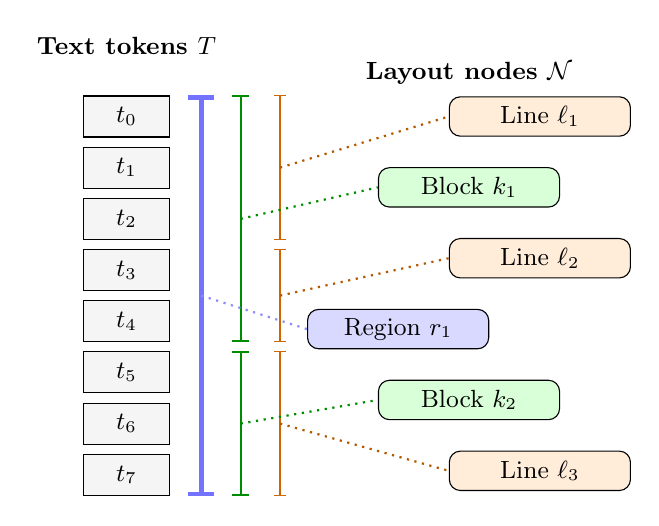
\begin{tikzpicture}[
      nd/.style={draw, rounded corners, font=\small, inner sep=3pt,
          minimum height=0.50cm, minimum width=2.3cm, text centered},
      tok/.style={draw, fill=gray!8, font=\small, inner sep=2pt,
          minimum height=0.52cm, minimum width=1.1cm, text centered},
      conn/.style={dotted, thick},
    ]

    % ---- Token column (LEFT, x = 0.55) ----
    \foreach \i/\lab in {
        0/$t_0$, 1/$t_1$, 2/$t_2$, 3/$t_3$,
        4/$t_4$, 5/$t_5$, 6/$t_6$, 7/$t_7$}{
        \node[tok] (T\i) at (0.55, {-\i*0.65}) {\lab};
      }
    \node[font=\small\bfseries, above=4mm of T0] {Text tokens $T$};

    % ---- Span brackets (MIDDLE) ----
    % Region r_1: [0,8)   outermost — x = 1.5
    \draw[|-|, ultra thick, blue!55]
    (1.5,  0.27) -- (1.5, {-7*0.65-0.27});
    % Block k_1: [0,5)  — x = 2.0
    \draw[|-|, thick, green!55!black]
    (2.0,  0.27) -- (2.0, {-4*0.65-0.27});
    % Block k_2: [5,8)
    \draw[|-|, thick, green!55!black]
    (2.0, {-5*0.65+0.27}) -- (2.0, {-7*0.65-0.27});
    % Line l_1: [0,3)  — x = 2.5
    \draw[|-|, orange!80!black]
    (2.5,  0.27) -- (2.5, {-2*0.65-0.27});
    % Line l_2: [3,5)
    \draw[|-|, orange!80!black]
    (2.5, {-3*0.65+0.27}) -- (2.5, {-4*0.65-0.27});
    % Line l_3: [5,8)
    \draw[|-|, orange!80!black]
    (2.5, {-5*0.65+0.27}) -- (2.5, {-7*0.65-0.27});

    % ---- Node column (RIGHT) ----
    % x position encodes hierarchy level:
    %   Region = 4.0 (leftmost), Block = 4.9, Line = 5.8 (rightmost)
    % y ordering by bracket midpoint to keep connectors crossing-free:
    %   l1 (mid=-0.65), k1 (-1.30), l2 (-2.275), r1 (-2.275), k2 (-3.9), l3 (-3.9)
    \node[nd, fill=orange!15] (L1) at (5.8,  0.00) {Line $\ell_1$};
    \node[nd, fill=green!15]  (K1) at (4.9, -0.90) {Block $k_1$};
    \node[nd, fill=orange!15] (L2) at (5.8, -1.80) {Line $\ell_2$};
    \node[nd, fill=blue!15]   (R)  at (4.0, -2.70) {Region $r_1$};
    \node[nd, fill=green!15]  (K2) at (4.9, -3.60) {Block $k_2$};
    \node[nd, fill=orange!15] (L3) at (5.8, -4.50) {Line $\ell_3$};
    % Section label centred above the node area
    \node[font=\small\bfseries] at (4.9, 0.55) {Layout nodes $\Nodes$};

    % ---- Connectors: bracket midpoint -> node.west ----
    % Diagonal lines; ordering above guarantees no crossings.
    \draw[conn, orange!70!black] (2.5, {-1.0*0.65}) -- (L1.west);  % l1: bracket mid y=-0.65
    \draw[conn, green!55!black]  (2.0, {-2.0*0.65}) -- (K1.west);  % k1: mid y=-1.30
    \draw[conn, orange!70!black] (2.5, {-3.5*0.65}) -- (L2.west);  % l2: mid y=-2.275
    \draw[conn, blue!45]         (1.5, {-3.5*0.65}) -- (R.west);   % r1: mid y=-2.275
    \draw[conn, green!55!black]  (2.0, {-6.0*0.65}) -- (K2.west);  % k2: mid y=-3.9
    \draw[conn, orange!70!black] (2.5, {-6.0*0.65}) -- (L3.west);  % l3: mid y=-3.9

  \end{tikzpicture}
  \caption{The alignment $\phi$ as a mapping from the token sequence $T$
    (left) to layout nodes (right).  Nested span brackets (centre) indicate
    which token range each node covers, colour-coded by hierarchy level:
    \textcolor{blue!70!black}{region} $\supset$
    \textcolor{green!60!black}{block} $\supset$
    \textcolor{orange!80!black}{line}.
    Containment ensures child brackets nest inside their parent; monotonicity
    ensures sibling brackets are non-overlapping.}
  \label{fig:alignment}
\end{figure}

\begin{remark}
  The optimal alignment problem reduces, at each level of $\LT$, to a
  \emph{monotone interval partition} of the parent's token span among its
  ordered children --- precisely the sub-problem solved by the DP algorithm
  described in \cref{sec:algo}.
\end{remark}

%% ---------------------------------------------------------------
\section{Alignment Algorithms}
\label{sec:algo}
%% ---------------------------------------------------------------

At each internal node $u$ of $\LT$, the alignment sub-problem is:
\begin{quote}
  \emph{Given $n$ ordered children $X = \langle x_0, \ldots, x_{n-1} \rangle$
  and the token sub-sequence $Y[a:b]$ already assigned to $u$, partition
  $[a, b)$ into $n$ contiguous, non-overlapping spans --- one per child ---
  maximising the total similarity score.}
\end{quote}
\noindent All three algorithms below solve this same sub-problem; they differ in
their optimality guarantee and time complexity.

%% ---
\subsection{Dynamic-Programming Alignment}
\label{sec:dp}

\paragraph{Formulation.}
Let $L = b - a$ denote the number of tokens available to the current
sub-problem.  We define two $(n \times (L{+}1))$ tables.  The score table
$J[i][k]$ stores the \emph{optimal total similarity} achievable by assigning
children $x_0, \ldots, x_i$ to the prefix $Y[a : a{+}k]$ of the available
tokens.  The pointer table $A[i][k]$ stores the corresponding optimal split
point $r$, i.e.\ the relative token index at which child $x_i$'s interval
begins, so that the full assignment can be recovered by traceback.

\paragraph{Recurrence.}
\[
  J[0][k] = \mathrm{sim}(x_0,\,[a,\,a{+}k)),
  \qquad k = 0, \ldots, L
\]
\[
  J[i][k] = \max_{0 \le r \le k}
  \Bigl( J[i{-}1][r] \;+\; \mathrm{sim}(x_i,\,[a{+}r,\,a{+}k)) \Bigr),
  \quad i \ge 1
\]
The optimal alignment is recovered by tracing $A$ from $(n{-}1, L)$ back to
$(0, \cdot)$.

\begin{figure}[h]
  \centering
  \hrule\vspace{4pt}
  \begin{minipage}{0.92\linewidth}
    \begin{algorithmic}[1]
      \Require children $X{=}\langle x_0,\ldots,x_{n-1}\rangle$,
      tokens $Y$, similarity $\mathrm{sim}$, bounds $a < b$
      \Ensure  intervals $\langle[a_0,b_0),\ldots,[a_{n-1},b_{n-1})\rangle$
      \State $L \gets b - a$
      \State Initialise $J[0..n{-}1][0..L] \gets -\infty$;\quad $A[0..n{-}1][0..L] \gets 0$
      \For{$k \gets 0$ \textbf{to} $L$}
      \State $J[0][k] \gets \mathrm{sim}(x_0,\, Y[a:a{+}k])$
      \EndFor
      \For{$i \gets 1$ \textbf{to} $n{-}1$}
      \For{$k \gets 0$ \textbf{to} $L$}
      \For{$r \gets 0$ \textbf{to} $k$}
      \State $s \gets J[i{-}1][r] + \mathrm{sim}(x_i,\, Y[a{+}r:a{+}k])$
      \If{$s > J[i][k]$}
      \State $J[i][k] \gets s$;\quad $A[i][k] \gets r$
      \EndIf
      \EndFor
      \EndFor
      \EndFor
      \State \textbf{Traceback:}\; $k \gets L$
      \For{$i \gets n{-}1$ \textbf{downto} $0$}
      \State $r \gets A[i][k]$;\quad $\mathrm{intervals}[i] \gets (a{+}r,\; a{+}k)$;\quad $k \gets r$
      \EndFor
      \State \Return $\mathrm{intervals}$
    \end{algorithmic}
  \end{minipage}
  \vspace{4pt}\hrule
  \caption{%
  \textbf{Optimal alignment via dynamic programming.}
  Given an ordered sequence of $n$ layout-tree children $X$ and a token
  sub-sequence $Y[a:b]$ of length $L = b - a$ already assigned to their
  parent node, the algorithm fills a score table $J[i][k]$ in which entry
  $(i, k)$ stores the maximum total similarity achievable by assigning
  children $x_0, \ldots, x_i$ to the first $k$ tokens $Y[a:a{+}k]$.
  A companion pointer table $A[i][k]$ records the optimal split point $r$
  for each entry, enabling the full assignment to be recovered in $O(n)$
  time by tracing $A$ from $(n{-}1, L)$ back to $(0, \cdot)$.
  The algorithm runs in $O(nL^2)$ time and $O(nL)$ space and is guaranteed
  to return the globally optimal monotone interval partition of $[a, b)$
  among the $n$ children.%
  }
  \label{alg:dp}
\end{figure}

\paragraph{Complexity and scalability.}
The triple nested loop (over $i$, $k$, and $r$) dominates the running time,
giving $O(nL^2)$ per call with $O(nL)$ space for the two tables.  While this
is optimal for the monotone interval-partition problem, it does not scale
to long documents: a page with $L = 500$ tokens and $n = 20$ children requires
$\sim\!2.5 \times 10^6$ similarity evaluations per DP call, and the cost
accumulates across all levels of $\LT$.  This motivates the greedy
approximation presented in \cref{sec:greedy}.

\begin{figure}[h]
  \centering
  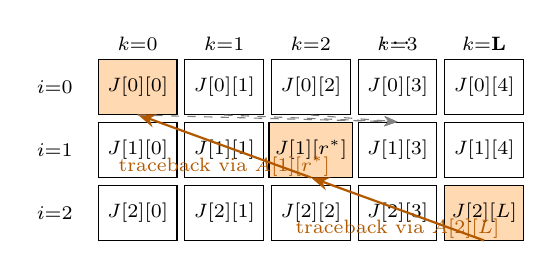
\begin{tikzpicture}[
      cell/.style={draw, minimum width=1.0cm, minimum height=0.7cm,
          font=\scriptsize, inner sep=2pt},
      highlight/.style={cell, fill=blue!18},
      traceback/.style={cell, fill=orange!30},
      arr/.style={->, >=Stealth, thick},
      dep/.style={->, >=Stealth, dashed, gray, thin},
    ]
    % Column headers (k)
    \foreach \k/\kl in {0/0, 1/1, 2/2, 3/3, 4/$L$} {
        \node[font=\scriptsize\bfseries] at ({1.1*\k}, 0.55) {$k{=}\kl$};
      }
    % Row headers (i)
    \foreach \i/\il in {0/$i{=}0$, 1/$i{=}1$, 2/$i{=}2$} {
        \node[font=\scriptsize\bfseries, left=2mm] at (-0.5, {-0.8*\i}) {\il};
      }

    % Grid cells
    \foreach \i in {0,1,2} {
        \foreach \k in {0,1,2,3,4} {
            \node[cell] (C\i\k) at ({1.1*\k}, {-0.8*\i}) {$J[\i][\k]$};
          }
      }

    % Traceback path highlight
    \node[traceback] at ({1.1*4}, {-0.8*2}) {$J[2][L]$};
    \node[traceback] at ({1.1*2}, {-0.8*1}) {$J[1][r^*]$};
    \node[traceback] at ({1.1*0}, {-0.8*0}) {$J[0][0]$};

    % Traceback arrows
    \draw[arr, orange!70!black]
    ({1.1*4}, {-0.8*2-0.35}) -- ({1.1*2}, {-0.8*1-0.35})
    node[midway, below, font=\scriptsize] {traceback via $A[2][L]$};
    \draw[arr, orange!70!black]
    ({1.1*2}, {-0.8*1-0.35}) -- ({1.1*0}, {-0.8*0-0.35})
    node[midway, below, font=\scriptsize] {traceback via $A[1][r^*]$};

    % Dependency arrows for J[1][3]
    \draw[dep] (C02.south) -- (C13.north);
    \draw[dep] (C01.south) -- (C13.north);
    \draw[dep] (C00.south) -- (C13.north);

    % Ellipsis column
    \node[font=\small] at ({1.1*3+0.0}, 0.55) {$\cdots$};
  \end{tikzpicture}
  \caption{Structure of the DP table $J$.  Each cell $J[i][k]$ is computed
    from all cells $J[i{-}1][r]$ with $r \le k$ (dashed arrows).  The
    traceback (orange) recovers the optimal split sequence from $J[n{-}1][L]$
    back to $J[0][0]$.}
  \label{fig:dp-table}
\end{figure}

%% ---
\subsection{Greedy Alignment}
\label{sec:greedy}

\paragraph{Motivation.}
When $L$ is large --- as is typical at the region or page level of a document
--- the $O(nL^2)$ DP becomes impractical.  The key observation motivating a
greedy approach is that, in well-structured documents, each layout node's
textual content is concentrated in a contiguous, roughly predictable region
of the token stream.  A locally committed forward scan therefore tends to
make accurate split decisions without requiring global optimisation.

\paragraph{Strategy.}
The algorithm maintains a cursor \texttt{pos}, initialised to $a$, which
marks the earliest token not yet assigned.  For each child $x_i$ in reading
order, it scans every candidate end position $k \in [\texttt{pos}, b]$,
evaluates $\mathrm{sim}(x_i, Y[\texttt{pos}:k])$, and irrevocably commits to
the $k$ that yields the highest score.  The final child $x_{n-1}$ is assigned
the remainder $[\texttt{pos}, b)$ unconditionally, ensuring full coverage of
the parent's span.

\begin{figure}[h]
  \centering
  \hrule\vspace{4pt}
  \begin{minipage}{0.92\linewidth}
    \begin{algorithmic}[1]
      \Require $X$, $Y$, $\mathrm{sim}$, $a$, $b$
      \Ensure intervals
      \State $\texttt{pos} \gets a$
      \For{$i \gets 0$ \textbf{to} $n{-}1$}
      \If{$i = n{-}1$}
      \State $\mathrm{intervals}[i] \gets (\texttt{pos},\, b)$;\quad \textbf{break}
      \EndIf
      \State $\textit{best\_score} \gets -\infty$;\quad $\textit{best\_k} \gets \texttt{pos}$
      \For{$k \gets \texttt{pos}$ \textbf{to} $b$}
      \State $s \gets \mathrm{sim}(x_i,\, Y[\texttt{pos}:k])$
      \If{$s > \textit{best\_score}$}
      \State $\textit{best\_score} \gets s$;\quad $\textit{best\_k} \gets k$
      \EndIf
      \EndFor
      \State $\mathrm{intervals}[i] \gets (\texttt{pos},\, \textit{best\_k})$
      \State $\texttt{pos} \gets \textit{best\_k}$
      \EndFor
      \State \Return $\mathrm{intervals}$
    \end{algorithmic}
  \end{minipage}
  \vspace{4pt}\hrule
  \caption{%
  \textbf{Greedy alignment.}
  The algorithm processes children $x_0, \ldots, x_{n-1}$ in reading order,
  maintaining a cursor \texttt{pos} that marks the start of the token range
  still available for assignment.
  For each child $x_i$, it scans every possible end position $k$ from
  \texttt{pos} to $b$ and commits irrevocably to the end point that
  maximises $\mathrm{sim}(x_i, Y[\texttt{pos}:k])$.
  The final child is assigned all remaining tokens $[\texttt{pos}, b)$
  unconditionally, guaranteeing full coverage of the parent span.
  Because each child requires at most $O(L)$ comparisons and there is no
  backtracking, the total time per call is $O(nL)$, making the greedy
  algorithm suitable for long token sequences where the quadratic DP cost
  would be prohibitive.
  Optimality is not guaranteed: an early greedy commit may allocate too
  many tokens to one child, leaving insufficient context for its siblings.%
  }
  \label{alg:greedy}
\end{figure}

\paragraph{Complexity and trade-offs.}
The algorithm performs a single forward pass with no backtracking, giving
$O(nL)$ time and $O(1)$ additional space (beyond the output).  Optimality is
not guaranteed: an early commit to an overlong span for $x_i$ can
``starve'' later children, leaving them with too few tokens to match their
content accurately.  In practice, accuracy is high when the similarity
function peaks sharply at the correct boundary and the content density across
children is roughly uniform --- conditions that hold for most well-typeset
academic documents.

%% ---
\subsection{Hybrid Strategy}
\label{sec:hybrid}

\paragraph{Design.}
The hybrid strategy dispatches to \cref{alg:dp} when the span length $L = b - a$
does not exceed a threshold $\theta$, and to \cref{alg:greedy} otherwise.
When $L \le \theta$, the DP cost is bounded by the constant $O(n\theta^2)$,
so the exact, globally optimal solution is obtained at negligible expense.
When $L > \theta$, the greedy algorithm's $O(nL)$ cost scales gracefully with
document length, preventing the quadratic blow-up that would occur with DP.
The threshold $\theta = 100$ is chosen empirically: paragraph-level
sub-problems in typical academic documents rarely exceed 100 tokens, while
page- or section-level spans regularly do.

\begin{figure}[h]
  \centering
  \hrule\vspace{4pt}
  \begin{minipage}{0.92\linewidth}
    \begin{algorithmic}[1]
      \Require $X$, $Y$, $\mathrm{sim}$, $a$, $b$;\quad threshold $\theta = 100$
      \Ensure intervals
      \If{$b - a > \theta$}
      \State \Return $\textsc{Greedy}(X, Y, \mathrm{sim}, a, b)$
      \Comment{$O(nL)$ --- large span, scalability preferred}
      \Else
      \State \Return $\textsc{DP}(X, Y, \mathrm{sim}, a, b)$
      \Comment{$O(nL^2)$ --- small span, optimality affordable}
      \EndIf
    \end{algorithmic}
  \end{minipage}
  \vspace{4pt}\hrule
  \caption{%
    \textbf{Hybrid alignment.}
    The hybrid strategy selects between the exact DP (\cref{alg:dp}) and the
    greedy approximation (\cref{alg:greedy}) based on the length $L = b - a$
    of the token span to be partitioned.
    When $L \le \theta$ (with $\theta = 100$), the span is short enough that
    the $O(nL^2)$ DP cost is bounded by the constant $O(n\theta^2)$, so the
    exact algorithm is used to obtain the globally optimal assignment.
    When $L > \theta$, the $O(nL)$ greedy algorithm is invoked instead,
    ensuring that the total alignment cost remains linear in the document
    length even for very long token sequences.
    The threshold $\theta = 100$ reflects the empirical observation that
    paragraph-level sub-problems in typical academic documents rarely exceed
    100 tokens, while page- or section-level spans often do.
    Applied recursively at every internal node of the Layout Tree $\LT$,
    the hybrid strategy automatically selects the exact solver for fine-grained
    levels (line $\to$ word) and the approximate solver for coarse levels
    (region $\to$ block), balancing accuracy and efficiency across the
    full document hierarchy.%
  }
  \label{alg:hybrid}
\end{figure}

\paragraph{Recursive application.}
The hybrid algorithm is invoked once at every internal node of $\LT$, with
the token span inherited from that node's own alignment serving as the
$[a, b)$ input.  At deeper levels of the tree --- such as line-to-word
partitioning --- the inherited spans are short and the DP branch dominates,
delivering exact solutions with negligible cost.  At shallower levels ---
such as region-to-block partitioning --- spans may encompass the full page,
and the greedy branch dominates, keeping the cost linear in the span length.
The overall time across all nodes of the tree is
$O\!\left(\sum_{u \in \LT} n_u L_u\right)$,
where $n_u$ is the number of children of node $u$ and $L_u = b_u - a_u$ is
the length of its assigned token span.  In the worst case this reduces to
$O(nL)$ for a balanced tree, matching the greedy algorithm's single-level cost.

%% ---------------------------------------------------------------
\section{System Implementation}
%% ---------------------------------------------------------------

The system is implemented as a Python library, \texttt{ppx}, that wraps
PaddleOCR and PPStructure\,V3 in a composable, type-safe pipeline.
\Cref{fig:system-arch} gives an overview of the two-phase architecture:
an \emph{offline processing} phase that ingests document images and
persists all derived artefacts to disk, and an \emph{online serving} phase
that exposes those artefacts through a REST API consumed by a web client.

\begin{figure}[h]
  \centering
  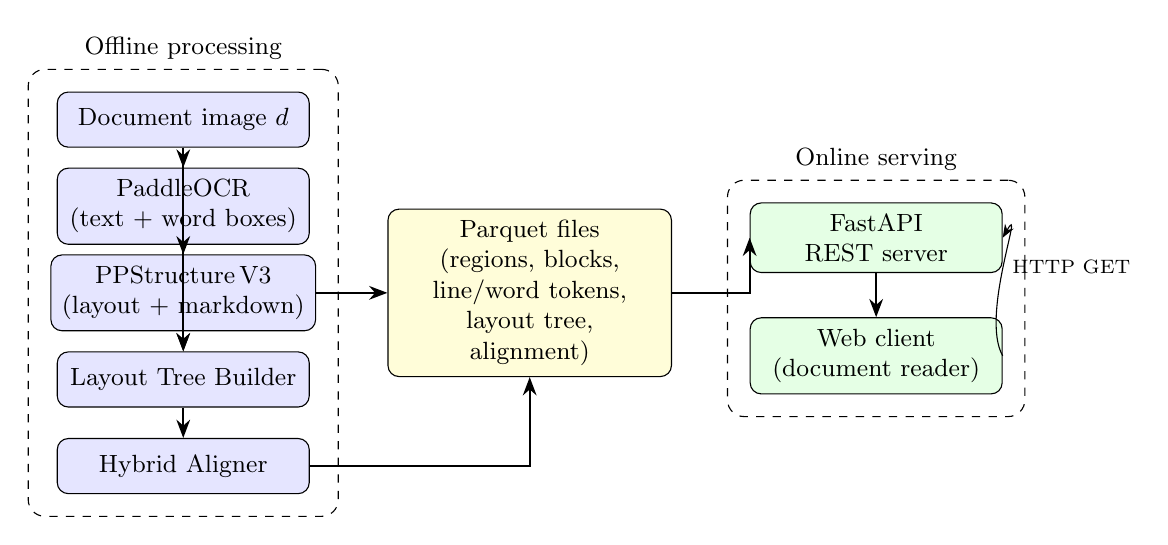
\begin{tikzpicture}[
      box/.style={draw, rounded corners, fill=white,
          minimum width=3.2cm, minimum height=0.7cm,
          font=\small, inner sep=4pt, align=center},
      store/.style={box, fill=yellow!15, minimum width=3.6cm},
      phase/.style={draw, dashed, rounded corners=6pt,
          inner sep=8pt, font=\small\bfseries},
      arr/.style={->, >=Stealth, thick},
      sarr/.style={->, >=Stealth},
    ]

    %% --- Offline column (left) ---
    \node[box, fill=blue!10]   (img)    at (0, 0)      {Document image $d$};
    \node[box, fill=blue!10]   (ocr)    at (0,-1.1)    {PaddleOCR\\(text + word boxes)};
    \node[box, fill=blue!10]   (ppstruct) at (0,-2.2)  {PPStructure\,V3\\(layout + markdown)};
    \node[box, fill=blue!10]   (tree)   at (0,-3.3)    {Layout Tree Builder};
    \node[box, fill=blue!10]   (aligner) at (0,-4.4)   {Hybrid Aligner};

    \draw[arr] (img)      -- (ocr);
    \draw[arr] (img)      -- (ppstruct);
    \draw[arr] (ocr)      -- (tree);
    \draw[arr] (ppstruct) -- (tree);
    \draw[arr] (tree)     -- (aligner);

    %% --- Data store (centre) ---
    \node[store] (store) at (4.4, -2.2)
    {Parquet files\\(regions, blocks,\\line/word tokens,\\layout tree,\\alignment)};

    \draw[arr] (aligner.east) -| (store.south);
    \draw[arr] (ppstruct.east) -- (store.west);

    %% --- Online column (right) ---
    \node[box, fill=green!10] (api)    at (8.8,-1.5) {FastAPI\\REST server};
    \node[box, fill=green!10] (client) at (8.8,-3.0) {Web client\\(document reader)};

    \draw[arr] (store.east) -| (api.west);
    \draw[arr] (api)   -- (client);
    \draw[sarr, bend left=20] (client.east) to[out=30,in=-30]
    node[right, font=\scriptsize]{HTTP GET} (api.east);

    %% --- Phase labels ---
    \begin{scope}[on background layer]
      \node[phase, fit=(img)(ocr)(ppstruct)(tree)(aligner),
      label=above:{\small Offline processing}] {};
      \node[phase, fit=(api)(client),
      label=above:{\small Online serving}] {};
    \end{scope}

  \end{tikzpicture}
  \caption{System architecture of the \texttt{ppx} document alignment pipeline.
    The offline phase ingests a raster document image, runs PaddleOCR for
    visual token extraction and PPStructure\,V3 for layout detection and
    Markdown generation, builds the Layout Tree, and computes the
    layout-text alignment.  All artefacts are persisted as Parquet files.
    The online phase serves these artefacts through a FastAPI REST server,
    which a browser-based web client queries to render the document with
    interactive alignment visualisation.}
  \label{fig:system-arch}
\end{figure}

%% ---
\subsection{PaddleOCR and PaddlePaddle Integration}
\label{sec:paddle}

PaddlePaddle is Baidu's open-source deep learning framework, optimised for
inference on both CPU and GPU hardware \cite{PaddleOCR30}.  PaddleOCR is
built on top of PaddlePaddle and provides pre-trained models for text
detection, recognition, and document layout analysis.  The system uses two
PaddleOCR entry points:
\begin{itemize}
  \item \texttt{PaddleOCR} --- the standard OCR pipeline, which detects text
        line bounding boxes and transcribes each line and its constituent
        words.
  \item \texttt{PPStructureV3} --- the document-structure pipeline, which
        additionally detects semantic regions (paragraphs, figures, tables,
        formulae), determines reading order, and converts the full page to
        Markdown.
\end{itemize}

Both models are computationally heavy to initialise; they are therefore
wrapped in Python's \texttt{functools.cache} to ensure that model weights are
loaded at most once per process:

\begin{lstlisting}
from functools import cache
from paddleocr import PaddleOCR, PPStructureV3

@cache
def get_ocr_model() -> PaddleOCR:
    return PaddleOCR(use_doc_unwarping=False)

@cache
def get_structv3_model() -> PPStructureV3:
    return PPStructureV3(use_doc_unwarping=False)
\end{lstlisting}

The \texttt{use\_doc\_unwarping=False} flag disables the perspective-correction
pre-processor, which is unnecessary for digitally-born PDF pages that are
already geometrically flat.  Both models are invoked with
\texttt{model.predict(np\_page)}, where \texttt{np\_page} is a
\texttt{numpy} array of shape $(H, W, 3)$ representing a single page image.

%% ---
\subsection{OCR and Layout Analysis Pipeline}
\label{sec:ocr-pipeline}

Each page is processed through two parallel inference calls that produce
complementary data layers.  The \texttt{get\_visual\_tokens} function
invokes the standard OCR model and parses its output into a
\texttt{VisualTokenLayers} dataclass containing a line-token DataFrame and a
word-token DataFrame.  Concurrently, \texttt{get\_structv3} invokes the
layout model and returns both a \texttt{LayoutLayers} dataclass (regions,
blocks, formulae) and a \texttt{MarkdownDocument} (the OCR-generated text
together with any extracted figure images):

\begin{lstlisting}
layout_layers, markdown_doc = get_structv3(np_page, page_index=i)
visual_layers = get_visual_tokens(np_page, page_index=i)
\end{lstlisting}

Both functions are decorated with \texttt{@memory.cache} (via
\texttt{joblib}), so repeated calls on the same page image are served from
disk without re-running inference --- a critical optimisation during
development and evaluation.

%% ---
\subsection{Type-Safe Data Representations}
\label{sec:types}

Every intermediate data product is represented as a \texttt{pandas}
DataFrame whose schema is declared and enforced by \texttt{pandera}.  Five
schema classes cover the full set of artefacts:

\medskip
\begin{center}
  \small
  \begin{tabular}{ll}
    \toprule
    Schema                   & Contents                                                       \\
    \midrule
    \texttt{LineTokenSchema} & Bounding box + transcribed text per OCR line                   \\
    \texttt{WordTokenSchema} & Bounding box + text + parent line index per word               \\
    \texttt{LayoutSchema}    & Bounding box + semantic label per layout region or element     \\
    \texttt{BlockSchema}     & Bounding box + label + reading-order index + content per block \\
    \texttt{FormulaSchema}   & Bounding box + \LaTeX\ formula text per detected formula       \\
    \bottomrule
  \end{tabular}
\end{center}
\medskip

Schema validation is applied at each pipeline boundary, so any type mismatch
or missing column is caught immediately rather than propagating silently into
downstream alignment code.  The \texttt{pandera} \texttt{DataFrame[Schema]}
type annotation also serves as machine-checked documentation, making the
expected column set explicit in every function signature.

%% ---
\subsection{Composable Pipeline Design}
\label{sec:composable}

Each processing stage is implemented as a \emph{pure function} that accepts
typed inputs and returns typed outputs with no hidden state.  The layout tree
is constructed by passing the four DataFrame layers from the two inference
calls to \texttt{build\_layout\_tree}:

\begin{lstlisting}
from ppx.core.layout.layout_tree import (
    build_layout_tree, get_largest_region, align_tree
)

tree_df = build_layout_tree(
    regions = layout_layers.regions,
    blocks  = layout_layers.blocks,
    lines   = visual_layers.line_tokens,
    words   = visual_layers.word_tokens,
)
root_id   = get_largest_region(tree_df)
alignment = align_tree(tree_df, root_id, markdown_doc.markdown)
\end{lstlisting}

Because each function is pure and its inputs are fully determined by its
arguments, the entire pipeline is trivially parallelisable across pages and
documents.  The \texttt{MarkdownDocument} dataclass bundles the Markdown text
with a dictionary mapping figure keys to extracted image arrays, keeping all
page artefacts together without coupling the layout and text pipelines.

%% ---
\subsection{Client/Server Architecture}
\label{sec:server}

The alignment artefacts produced offline are persisted as Apache Parquet
files --- one directory per page, containing separate \texttt{.parquet}
files for regions, blocks, line tokens, word tokens, the layout tree, and
the alignment JSON.  This storage layout decouples ingestion from serving:
new documents can be added to the data directory without restarting the
server.

The online serving layer is a \texttt{FastAPI} application that maps HTTP
GET requests to artefact reads:

\begin{lstlisting}
@router.get("/documents/{filename}/pages/{page_index}/alignment")
def get_alignment(filename: str, page_index: int) -> dict:
    page_dir  = _resolve_page(filename, page_index)
    alignment = TreeAlignment.model_validate_json(
        (page_dir / "alignment.json").read_text()
    )
    return alignment.model_dump()
\end{lstlisting}

The server exposes endpoints for listing documents, retrieving per-page
images and Markdown, fetching raw visual token layers, and returning the
pre-computed layout tree and alignment.  A browser-based web client queries
these endpoints and renders the document with interactive alignment
visualisation: clicking a text span highlights the corresponding bounding
boxes on the page image, and hovering a bounding box highlights the aligned
text span.  The server is launched via \texttt{uvicorn} and accepts a
\texttt{--data} directory argument, making deployment to any POSIX host
straightforward.

%% ---------------------------------------------------------------
\section{Experiments}
%% ---------------------------------------------------------------

\subsection{Dataset and Setup}
\begin{itemize}
  \item Document corpus: academic paper page images processed via PaddleOCR
        \cite{PaddleOCR30} and PP-DocLayout \cite{PPDocLayout}
  \item Baseline comparison: SCAN semantic layout analysis \cite{scan2025semantic}
  \item Metrics: token-span accuracy, character-span overlap ratio
\end{itemize}

\subsection{Results}

%% ---------------------------------------------------------------
\section{Conclusion}
%% ---------------------------------------------------------------
\begin{itemize}
  \item Summary of contributions: formal model, hybrid aligner, composable pipeline
  \item Limitations and future work
\end{itemize}

% References
\bibliographystyle{unsrtnat}
\bibliography{references}

\end{document}
